\section{Experimental Environment}
\label{sec:experimental-environment}

To test the efficiency of the selected tools, a designated Kuberntes environment was created. We have chosen Rancher Desktop for provisioning a local instance of Kubernets. Then, a simple demo application, preemptively exposed with vulnerabilities was deployed inside this cluster. It includes two interconnected microservice apps, simulating a simple solution for user and subject management. Each application is composed of a simple Spring Boot Java application, NextJS frontend and a PostgreSQL database. We have chosen Spring Boot, ReactJS and PostgreSQL as these are the most popular technologies for miscroservice applications nowadays. Business logic of these application is simple and is irrelevant to our purpose. Figure~\ref{img:demo-apps} capture the user interface of those applications. We made \textbf{demo-users} application as insecure as possible, while leaving \textbf{demo-subjects} application without any explicit security configuration. In this section we describe the features of the environment, while mapping some of the security threats from the Section~\ref{sec:security-threats-classification} to their implementation in the configuration files.

\begin{figure}[!hbt]
	\centering
  \begin{subfigure}[b]{0.45\textwidth}
		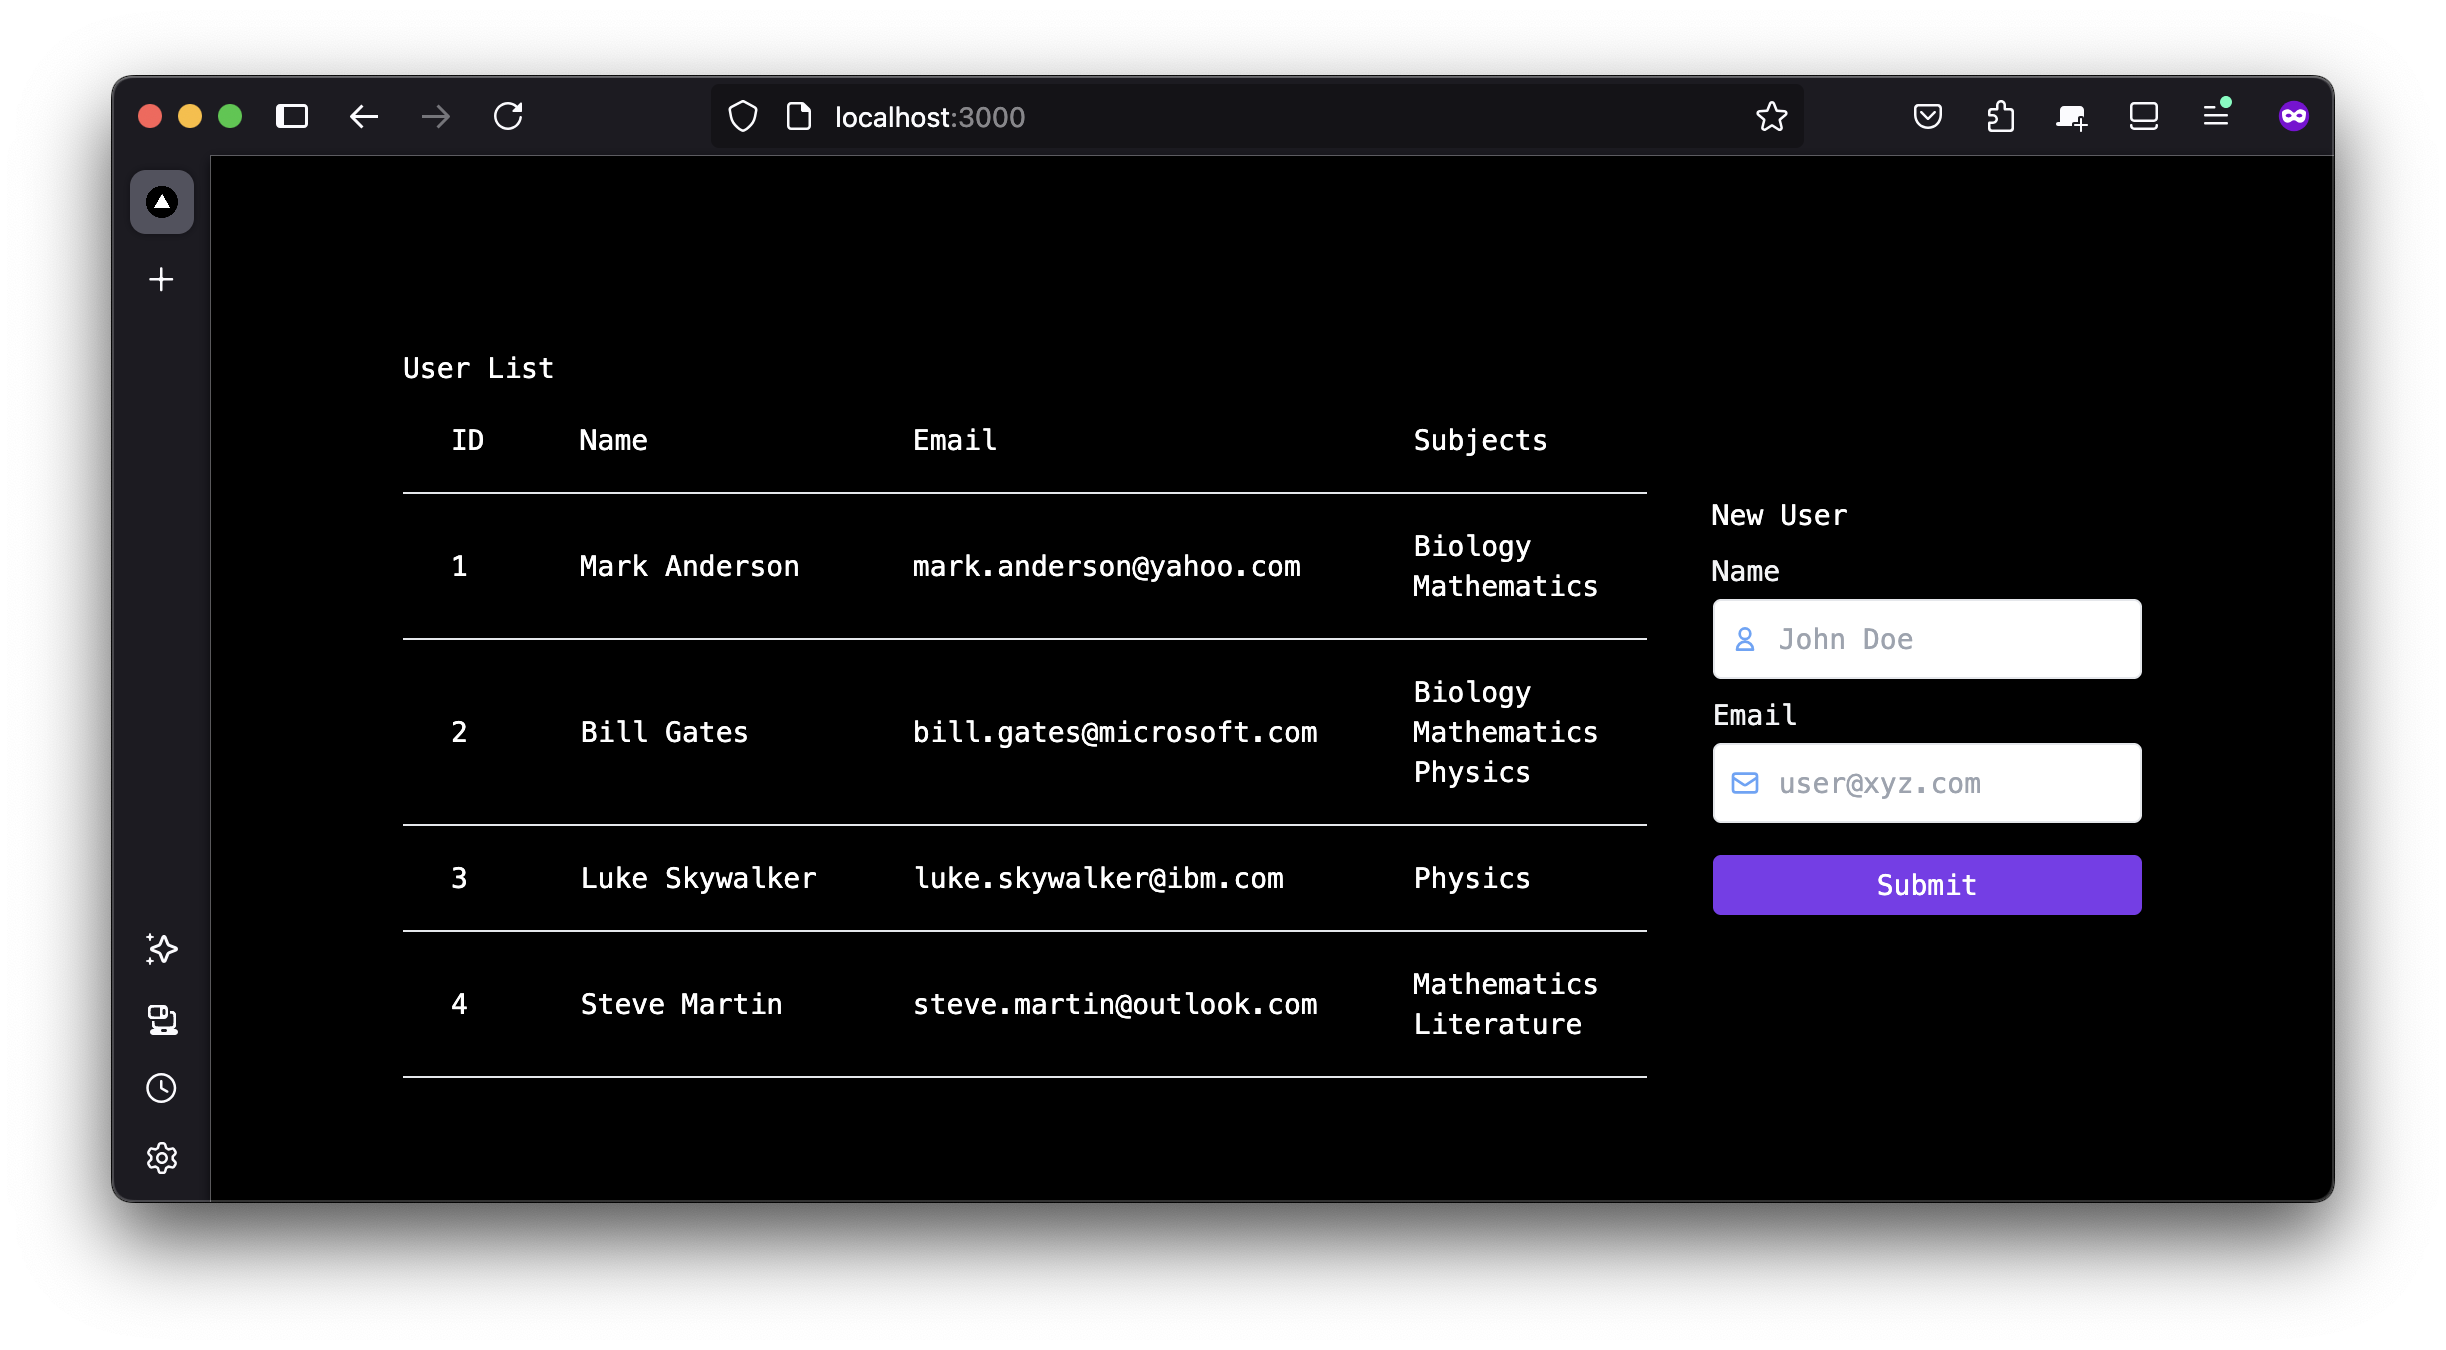
\includegraphics[width=1.1\linewidth]{images/demo-users.png}
        \caption{\textbf{demo-users} application.}
		\label{img:demo-users}
  \end{subfigure}
  \hfill
  \begin{subfigure}[b]{0.45\textwidth}
		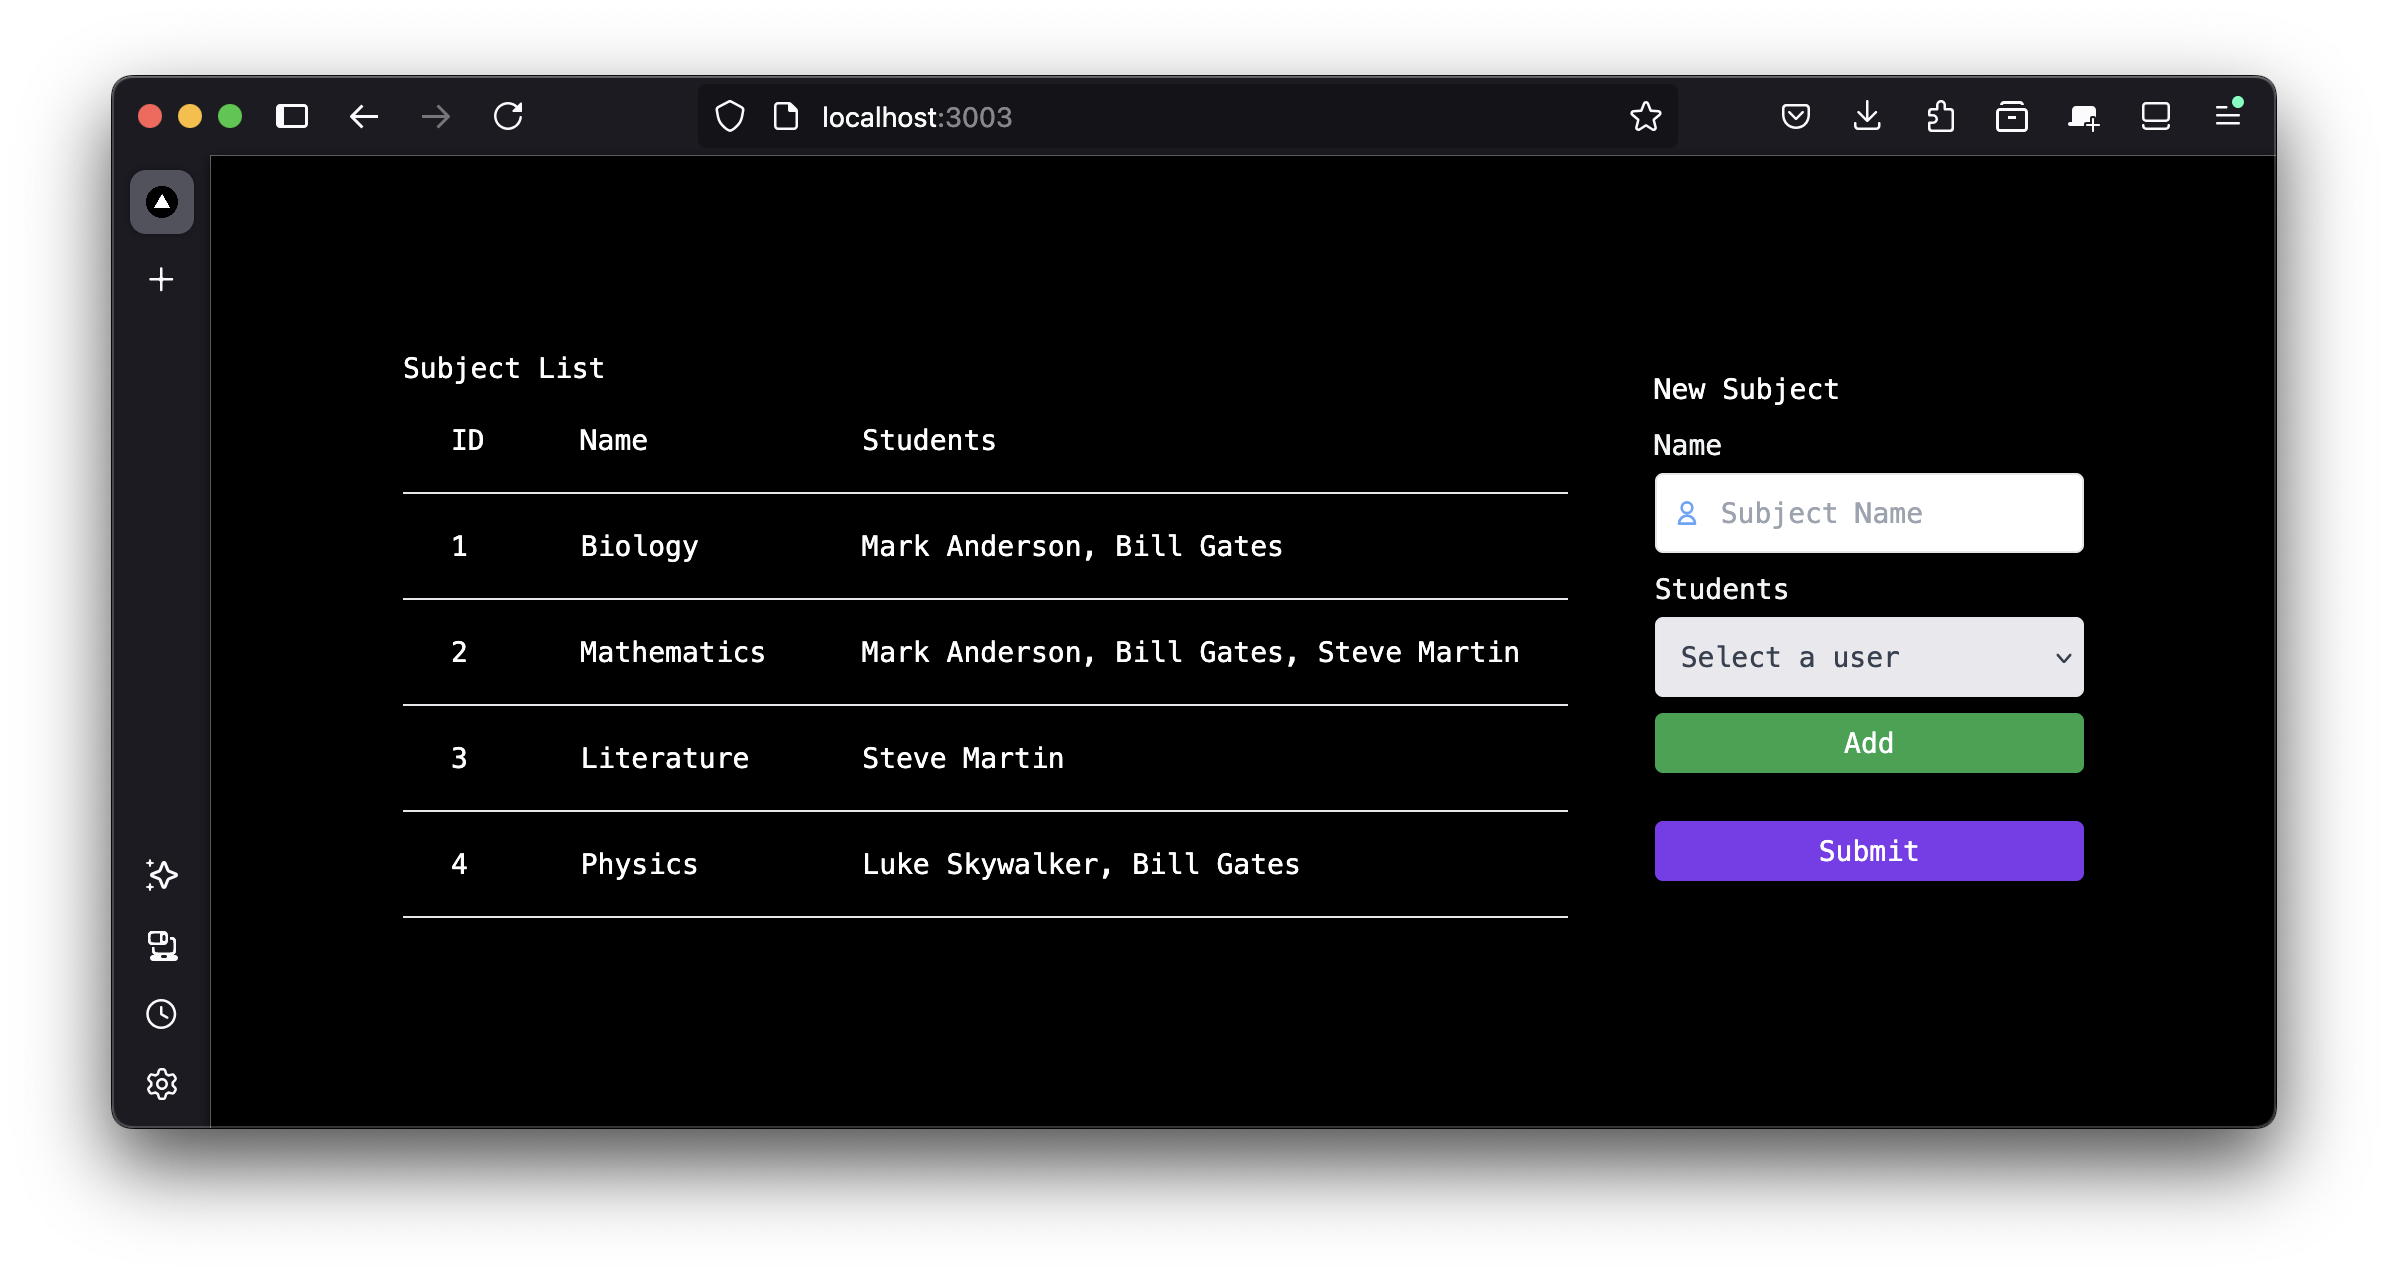
\includegraphics[width=1.1\linewidth]{images/demo-subjects.png}
        \caption{\textbf{demo-subjects} application.}
		\label{img:demo-subjects}
  \end{subfigure}
  \caption{Demo applications.}
  \label{img:demo-apps}
\end{figure}

\subsection{Cluster and Namespaces}

For our test we used the most recent Kubernetes version 1.32.0. We leave the Kubernetes API on the default 6443 port and use dockerd as the container engine in Rancher Desktop. Apart from that, no additional configuration is needed for the cluster setup.

We label the \textbf{demo-users} namespace with
\begin{center}
  \lstinline|pod-security.kubernetes.io/enforce=privileged|,
\end{center} 
which enforces the rule that any pod running in that namespace must be configured with elevated privileges. Privileged containers can access the host system's devices, and resources like \lstinline{/dev} or \lstinline{/sys} that are normally restricted in regular containers. They may be granted additional Linux capabilities (such as \lstinline{SYS_ADMIN} or \lstinline{NET_ADMIN}), allowing the container to perform actions that are typically restricted (e.g., managing network interfaces, mounting file systems, etc.).

\subsection{Docker Images}

To make the images less secure, we have avoided any reecommendations for the Docker image security. That is, for \textbf{demo-users} we run the images as root by default. We explicitly expose ports 9229 (NodeJS debug port) and 22 (SSH port) to open them up for a potentional attack. Additionally, we define environment variables containing sensitive information. Finally, we use \lstinline{latest} image tag, so that the image with undeterministic nde version and potentially unpatched vulnerabilities is used for the build. Listing~\ref{lst:demo-users-dockerfile} demonstrates the Dockerfile for the \textbf{demo-users} frontend image.

\begin{lstlisting}[language=Dockerfile, caption={[Demo-users frontend image]\textbf{demo-users} frontend image.}, label={lst:demo-users-dockerfile}]
    # use the latest image from Dockerhub
    # use image tag instead of hash
    FROM node:latest
    
    WORKDIR /app
    
    COPY package*.json ./
    RUN npm ci
    
    COPY . ./
    COPY entrypoint.sh /app/entrypoint.sh
    RUN npm run build && \
        chmod +x /app/entrypoint.sh
    
    # sensitive information in environment variables
    ENV AUTH_TOKEN=QmVhcmVyIHh3SmRhMDl4T0NhNWFQUXpxM2NjeHF3Vwo=
    
    EXPOSE 3000
    # expose unnecessary ports
    EXPOSE 9229 22
    
    # run as root
    USER root
    
    ENTRYPOINT /app/entrypoint.sh
\end{lstlisting}

\subsection{Helm Charts}

Vast majority of the misconfigurations belong to the Helm charts. We explicitly grant the cluster administrator rights to the ServiceAccount running the \textbf{demo-users} Deployment (see Listing~\ref{lst:demo-users-rbac}). This means that a potential attacker obtains full cluster control if he gets access to the pod. Then, we do not restrict or limit the CPU and memory resources available to the pod. Thus, a pod can, potentially, exhaust the node resources, significantly disrupting critical workload availability. We do not define any preemption policies, which makes Kubernetes scheduler treat our workloads as the same priority class. Lastly, we explicitly grant the containers all Linux capabilities, making the root filesystem writable and enforce root user to run the containers. Listing~\ref{lst:demo-users-security-context} provides a snippet from the Helm values, which define some of the security configuration parameters.

\begin{lstlisting}[language=YAML, caption={[RoleBinding definition for demo-users ServiceAccount] RoleBinding definition for \textbf{demo-users} ServiceAccount, granting it cluster administrator rights.}, label={lst:demo-users-rbac}]
apiVersion: rbac.authorization.k8s.io/v1
kind: RoleBinding
metadata:
  name: {{ include "demo.serviceAccountName" . }}-rolebinding
subjects:
- kind: ServiceAccount
  name: {{ include "demo.serviceAccountName" . }}
  namespace: {{ .Release.Namespace }}
roleRef:
  kind: ClusterRole
  # 1.1. Misconfigured RBAC
  name: cluster-admin
  apiGroup: rbac.authorization.k8s.io
\end{lstlisting}

\begin{lstlisting}[language=YAML, caption={[Demo-users Helm Chart values snippet] \textbf{demo-users} Helm Chart values snippet, granting the container unnecessary permissions.}, label={lst:demo-users-security-context}]
# 6.1 and 6.2
securityContext: {}
  capabilities:
    add:
    - ALL # Grants all capabilities to the container
  # Allows the root filesystem to be writable
  readOnlyRootFilesystem: false 
  runAsNonRoot: false # Allows the container to run as root
  runAsUser: 0 # Runs the container as the root user
\end{lstlisting}